\chapter{Gradient descent}

\section{Model based machine learning}
Nel model based machine learning si sceglie un modello definito da un insieme di parametri.
In particolare si nota come:
\begin{multicols}{2}
	\begin{itemize}
		\item Per i decision trees i parametri sono la struttura dell'albero, quali features ogni nodo divide e le predizioni delle foglie.
		\item Per il perceptron i parametri sono i pesi e il valore di $b$.
	\end{itemize}
\end{multicols}
Dopo aver scelto il modello si deve scegliere un criterio da ottimizzare o la funzione obiettivo come per esempio il training error.
Infine si sviluppa un algoritmo di learning che deve cercare di minimizzare il criterio, spesso in maniera euristica.

	\subsection{Modelli lineari}
	Nei modelli lineari il modello \`e:
	$$0=b+\sum\limits_{j=1}^mw_jf_j$$
	Si deve scegliere il criterio da ottimizzare.

		\subsubsection{Notazioni}
		
		\paragraph{Funzione indicatrice}
		Una funzione indicatrice trasforma valori di \emph{Vero} e \emph{Falso} in numeri e li conteggia.
		$$1[x]=\begin{cases}1&\mathbf{if}\ x = True\\
			0&\textbf{if}\ x = False
		\end{cases}$$
		
		\paragraph{Dot-product}
		Utilizzando una notazione vettoriale si rappresenta un esempio $f_1,\dots,f_m$ come un vettore singolo $\overrightarrow{x}$ in cui $j$ indicizza la feature e $i$ indicizza un dataset di esempi.
		Si possono rappresentare anche i pesi $w_1,\dots,w_m$ come un vettore $\overrightarrow{w}$.
		Il dot-product tra due vettori $a$ e $b$ viene definito come:
		$$a\cdot b = \sum\limits_{j=1}^ma_jb_j$$
		
		\subsubsection{Funzione obiettivo}
		Il criterio da ottimizzare o funzione obiettivo pu\`o essere:
		$$\sum\limits_{i=1}^n1[y_i(w\cdot x_i+b)\le 0]$$
		A parole questa funzione conta quante volte la predizione \`e diversa dalla verit\`a. 
		Si devono pertanto trovare $w$ e $b$ tali che minimizzano questa funzione, ovvero:
		$$argmin_{w,b}\sum\limits_{i=1}^n1[y_i(w\cdot x_i+b)\le 0]$$

\section{Loss functions}

	\subsection{Loss $0/1$}
	Una funzione di loss $0/1$ \`e una funzione nella forma:
	$$\sum\limits_{i=1}^n1[(y_i(w\cdot x_i+b)\le 0]$$
	Dove tra le quadre si trova se la predizione e la label sono d'accordo, con vero se non lo fanno e tra le tonde la distanza dall'iperpiano, di cui il segno \`e la predizione.
	Questa funzione ritorna il numero di errori nella predizione.

		\subsubsection{Minimizzare la loss $0/1$}
		Per minimizzare una funzione $0/1$ si deve, ogni volta cambiare un valore di $w$ in modo che l'esempio \`e corretto o scorretto la perdita aumenta o diminuisce.
		Si nota come a ogni feature aggiunta si aggiunge una nuova dimensione allo spazio.
		Per il minimo si cercano $w$ e $b$ che minimizzano la perdita.
		Questo \`e un problema \emph{NP-hard}.
		Sue difficolt\`a comprendono il fatto che piccoli cambi in ogni $w$ possono portare a grandi cambi nella perdita in quanto il cambio non \`e continuo. 
		Inoltre trovare il minimo \`e complicato perch\`e non \`e differenziabile.
		Ci possono essere molti minimi locali.
		Ad ogni punto non si hanno informazioni che direzionano verso il minimo.
		Pertanto si nota come una loss function ideale sia continua e differenziabile in modo da avere un'indicazione verso la direzione di minimizzazione e un unico minimo, dunque unici $b$ e $w$.
		
		\paragraph{Loss function ideale}
		Una loss function ideale dovrebbe essere:
		\begin{itemize}
			\item Continua in modo da ottenere informazioni riguardo la direzione della minimizzazione.
			\item Avere un solo minimo.
			\item Misurare la distanza tra la predizione reale e quella predetta.
		\end{itemize}

	\subsection{Funzioni convesse}
	In una funzione convessa il segmento tra qualsiasi due punti della funzione si trova al di sopra della funzione.

	\subsection{Surrogate loss function}
	Per molte applicazioni si vuole minimizzare la loss $0/1$.
	Una surrogate loss function \`e una loss function che fornisce un limite superiore alla loss function attuale. 
	Dunque abbassando la surrogate loss stiamo abbassando anche la loss.
	Si vuole identificare un surrogato convesso della loss function in modo da facilitarne la minimizzazione.
	Chiave a una loss function \`e come verifica la differenza tra la label $y$ effettiva e la predizione $y'$.
	
		\subsubsection{Alcune surrogate loss function}
		
		Rappresentazione grafica in figura \ref{fig:chapter08-00}.
		Ricorda che: $y' = w \cdot x + b$ e $y \in \{-1,+1\}$.
		\begin{multicols}{2}
			\begin{itemize}
				\item \emph{$0/1$ loss}: $l(y, y')=1[yy'\le 0]$.
				\item \emph{Hinge} $l(y,y')=\max(0,1-yy')$, utilizzato nelle SVM.
				\item Exponential: $l(y,y')=\exp(-yy')$
				\item \emph{Squared loss}: $l(y,y')=(y-y')^2$.
			\end{itemize}
		\end{multicols}
		
		\begin{figure}
			\centering
			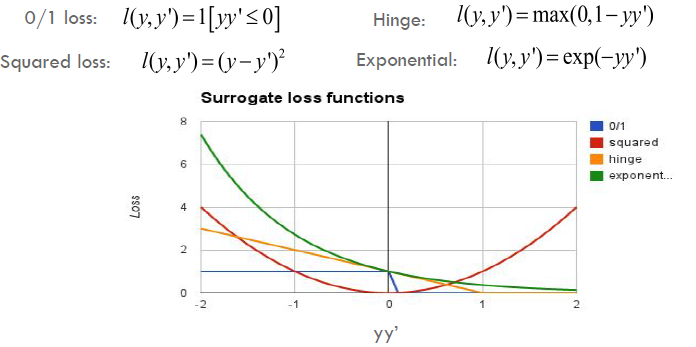
\includegraphics[width=0.6\linewidth]{imgs/chapter8/img0}
			\caption{Surrogate loss functions}
			\label{fig:chapter08-00}
		\end{figure}

		\subsubsection{Model-based machine learning}
		\begin{itemize}
			\item Prendi un modello 
			$$0=\sum\limits_{i=1}^m{w_i f_i}$$
			\item Scegli un criterio da ottimizzare, utilizzando una surrogate convex loss function:
			$$\sum\limits_{i=1}^n{exp(-y_i (w\cdot x_i+b))}$$
			\item Sviluppa un algoritmo di learning, che trovi $w$ e $b$ che minimizzano la surrogate loss: 
			$$argmin_{w,b}\sum\limits_{i=1}^n{exp(-y_i (w\cdot x_i+b))}$$
		\end{itemize}

\section{Gradient descent}
Il gradient descent \`e un modo per trovare il minimo locale o globale di una funzione: le derivate parziali danno un slope o direzione dove muoversi in tale dimensione.
Questo approccio consiste di scegliere un punto di partenza e a ripetizione di: scegliere una dimensione e muoversi di una piccola quantit\`a verso il minimo utilizzando la derivata. 
Questo algoritmo viene utilizzato per minimizzare la loss function.
Pertanto si:
\begin{itemize}
	\item Sceglie un punto di inizio $w$.
	\item Sceglie una dimensione.
	\item Si muove di una piccola quantit\`a verso la diminuzione della loss utilizzando la derivata.
\end{itemize}
Questo ciclo si ripete fino a che la loss non diminuisce in nessuna dimensione.

	\subsection{Spostamento in direzione della minimizzazione dell'errore}
	Il movimento in direzione della minimizzazione dell'errore \`e pertanto:
	$$w_j = w_j - \eta \dfrac{d}{dw_i}loss(w)$$
	Dove $\eta$ \`e il learning rate, \`e un iperparametro che regola di quanto muoversi nella direzione del minimo, e quindi quanto \`e aggressivo il training, tipicamente cambia nel corso del training.
	Notiamo che viene fatta una sottrazione perch\`e intendiamo andare verso il minimo della funzione.

		\subsubsection{Calcolo dello spostamento per la loss function esponenziale}
		Si deve pertanto calcolare la loss su tutto il training set:
		\begin{align*}
			\dfrac{d}{dw_j}loss &=\dfrac{d}{dw_j}\sum\limits_{i=1}^n\exp(-y_i(w\cdot x_i + b))=\\
			&=\sum\limits_{i=1}^n\dfrac{d}{dw_j}[-y_i(w\cdot x_i+b)]\exp(-y_i(w\cdot x_i+b))\\
		\end{align*}
		Si consideri pertanto ora:
		\begin{align*}
			\dfrac{d}{dw_j}[-y_i(w\cdot x_i + b)]&=-\dfrac{d}{dw_j}[y_i(w\cdot x_i + b)]=\\
			&=-\dfrac{d}{dw_j}y_i(\sum_{j=1}^{m}w_jx_{ij}+b)=\\
			&=-\dfrac{d}{dw_j}y_i(w_1x_{i1}+\cdots+w_mx_{im}+b)=\\
			&=-y_ix_{ij}
		\end{align*}
		Si nota pertanto come:
		$$\dfrac{d}{dw_j}loss=\sum\limits_{i=1}^n-y_ix_{ij}\exp(-y_i(w\cdot x_i+b))$$
		Si aggiorna pertanto $w_j$:
		$$w_j=w_j-\eta\sum\limits_{i=1}^n-y_ix_{ij}\exp(-y_i(w\cdot x_i+b))$$
		Questo viene fatto per ogni esempio $x_i$.

	\subsection{Learning algorithm del perceptron}
	Si nota pertanto come considerando il perceptron nell'ambito del gradient descent si aggiorna sempre il vettore dei pesi.\\
	\begin{algorithm}[H]
\DontPrintSemicolon
\SetKwComment{comment}{$\%$}{}
\SetKw{Int}{int}
\SetKw{To}{to}
\SetKw{IsNot}{is not}
\SetKw{Not}{not}
\SetKwData{Item}{item}
\SetKwFunction{Min}{min}
\SetKwFunction{Perceptron}{Perceptron}

\caption{\protect\Perceptron{}}

\Repeat{Convergence}{
	\ForEach{training example ($f_1, f_2,\dots,f_n, label$)}{
		\comment{Label = $\pm 1$}
		$prediction\ =\ b\ +\ \sum\limits_{i=1}^nw_if_i$\;
			\ForEach{$w_i$}{
				$w_j = w_j + \eta y_ix_{ij}\exp(-y_i(w\cdot x_i + b))$
			}
		$b\ =\ b\ +\ label$\;
		}
	}



\end{algorithm}

	Si noti come in questo caso $\eta$ rappresenta il learning rate, $y_i$ la label e $(w\cdot x_i + b))$ la predizione.
	Questi generano una costante $c$

	\subsection{Costante $\mathbf{c}$}
	Nella costante $c$ se label e predizione hanno lo stesso segno quando gli elementi predetti aumentano gli aggiornamenti diventano minori.
	Se invece sono diversi pi\`u diversi lo sono, maggiore l'aggiornamento.
	
	\subsection{Gradiente}
	Il gradiente \`e il vettore delle derivate parziali rispetto a tutte le dimensioni:
	$$\nabla L = \biggl[\dfrac{\partial L}{\partial w_1}\cdots\dfrac{\partial L}{\partial w_N}\biggr]$$
	Ogni derivata parziale misura quanto veloce ci muoviamo verso il minimo in una certa dimensione.
	Quando il gradiente \`e zero la loss non cambia in nessuna direzione.\\
	\input{Pseudocodice/09_gradient_descent}
	Nota come la funzione prenda in ingresso una lista di learning rate $\eta$, perch\`e potremmo voler cambiare il learning rate pi\`u ci avviciniamo al minimo, facendo passi grandi quando ci troviamo distanti e piccoli quando siamo vicini.
	Nei problemi in cui il problema di ottimizzazione \`e non convesso si trovano dei minimi locali \ref{fig:chapter08-01}, questi non permettono all'algoritmo di proseguire in quanto non distingue tra minimi locali e minimi globali.
	Un altro punto \`e un punto a sella, in cui certe direzioni curvano verso l'alto e altre verso il basso.
	In tali punti il gradiente \`e $0$ e l'algoritmo si blocca.
	Un modo per uscire da un punto \`a sella \`e spostarsi a lato un po' in modo da uscirne.
	Si nota come i punti a sella sono molti comuni in alte dimensioni.
	Il learning rate \ref{fig:chapter08-02} \`e molto importante in quanto permette di decidere la distanza coperta da uno spostamento determinando velocit\`a di avvicinamento al minimo e precisione dell'algoritmo.
	
	\begin{figure}
		\centering
		\begin{minipage}{.5\textwidth}
			\centering
			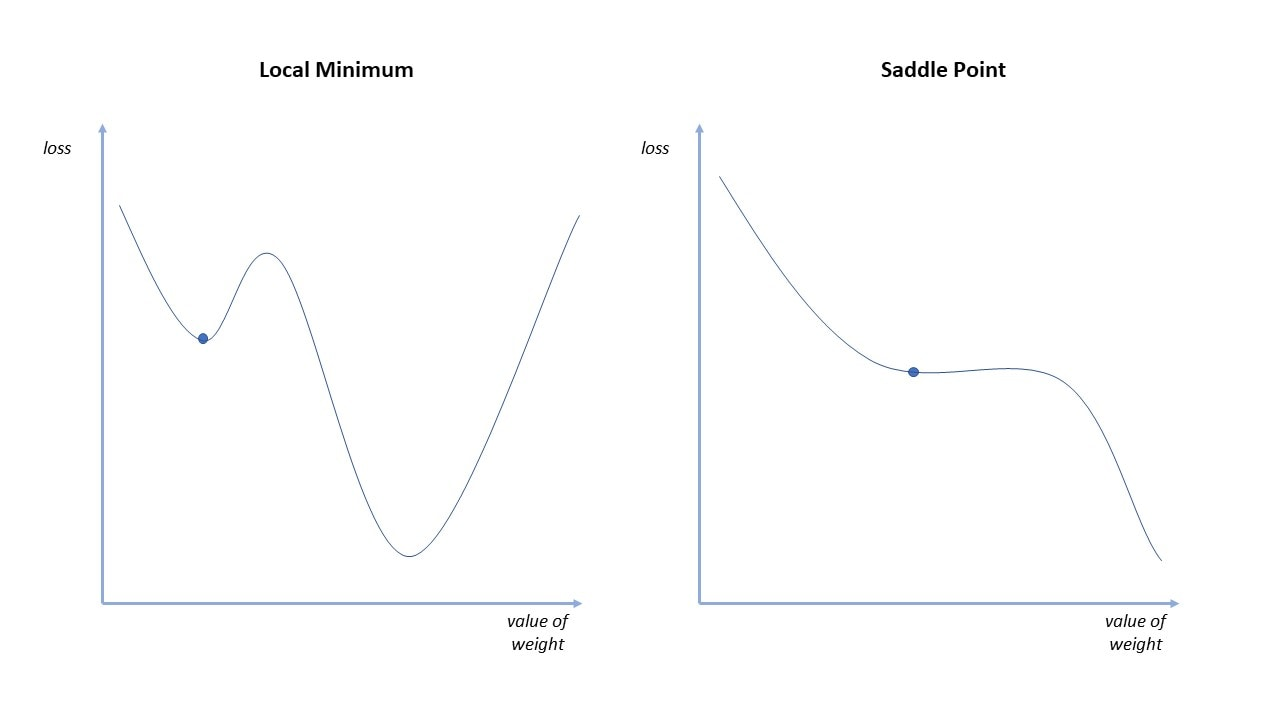
\includegraphics[width=1\linewidth]{imgs/chapter8/img1}
			\caption{Gradient descent}
			\label{fig:chapter08-01}
		\end{minipage}%
		\begin{minipage}{.5\textwidth}
			\centering
			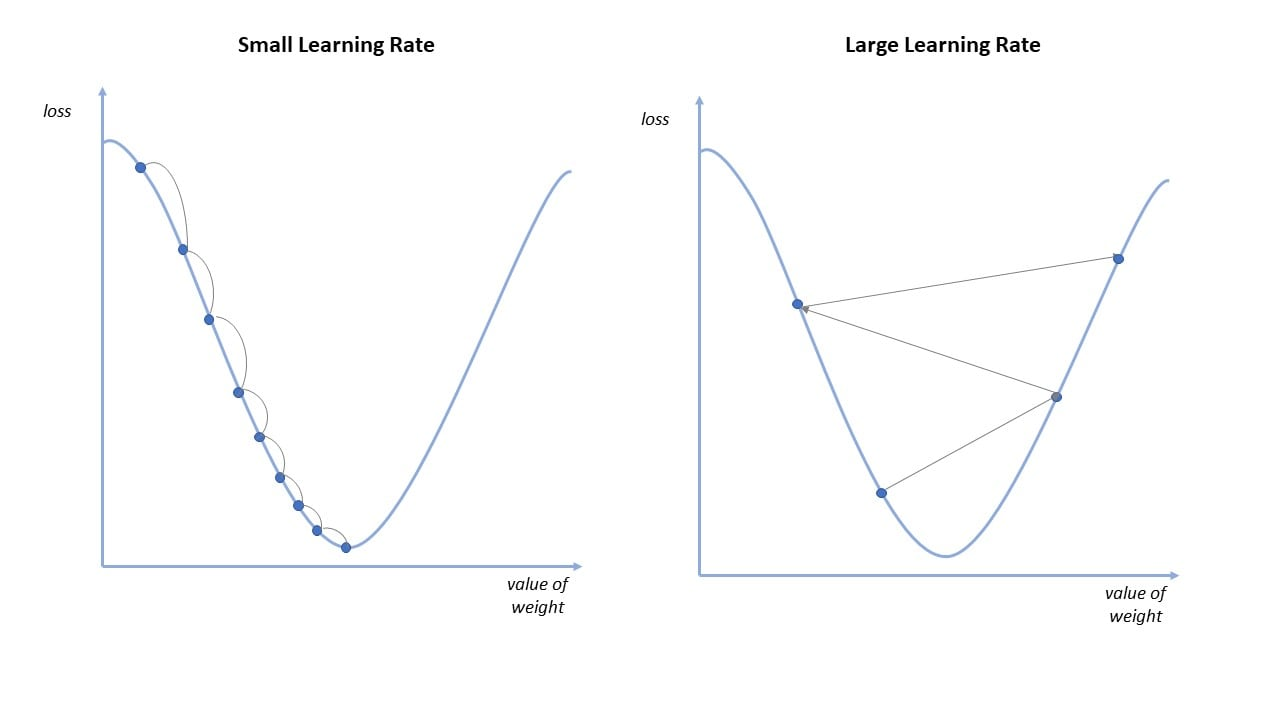
\includegraphics[width=1\linewidth]{imgs/chapter8/img2}
			\caption{Con un learing rate basso dovremo fare tanti passi per raggiungere il minimo, con uno alto potremmo trovarci ad oscillare.}
			\label{fig:chapter08-02}
		\end{minipage}
	\end{figure}

